\chapter{Regional Management}\label{chapter:RegionalManager}

The management of a hydrologic system can be achieved by controlling
releases at critical structures. For example, water levels in
reservoirs can be managed with regulation schedules, where the
controlled releases at the reservoir's inlet and outlet structures are
based on the state of the system and calendar date. Likewise, water
levels in canals can be managed using stage based operations where
gate openings start to open or close depending on threshold water
levels in the canal. In either case, the release through the
respective structures are constrained to achieve a managment
objective.

The RSM uses Regional Managers to compute and impose constraints on
selected structures in the simulated hydrologic system. For example,
water supply shortage plans are implemented through regional
managers. If the service area is under drought conditions, water
supply releases to the basins in the service are cutback by setting
management constraints on the corresponding structures. The RSM also
provides a generic mechanism whereby management constraints can be
applied to selected structures using decision trees. For example, a
lake regulation schedule comprised of management zones can be
transformed into a decision tree structure, where hydrologic
conditions are tested against the hydrologic criteria of each
management zone to determine which (if any) of the prescribed
operations (i,e., constraints) should be applied to the corresponding
structure.

The relative position of the regional managers to other computational
processes in the RSM (see Figure \ref{rsmFlowchart} has important
implications. The position of the regional manager processing
determines (1) what information is available for computing a
management constraint and (2) which processes can be subject to
management constraint. For example, if a release in an HPM is to be
controlled by a management constraint, the regional manager must be
processed before the HPMs. Given the sequential programming structure
of the RSM, this limits the data available to this regional manager to
assessors from the previous time step and the beginning of the time
step state variables. Delaying regional manager processing to just
before the HSE iteration adds data from the processed HPMs and
assessors. The computed management constraint can be used in
subsequent processes but are not updated in the HSE iteration loop.

Regional Managers use different mechanisms to compute and impose
management constraints on selected structures during the
simulation. Water supply management plans are implemented using a
single module that computes and applies the management constraints on
the associated water supply structures. The decision tree modules
compute the contraint values and place the results in designated
places to be used by other processes that actually apply the
constraint.

\begin{figure}
 \begin{center}
  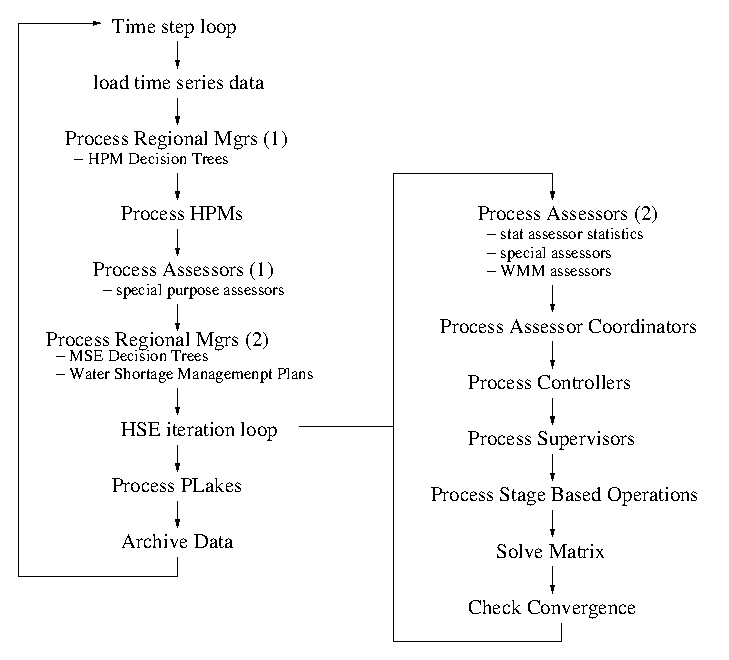
\includegraphics[scale=.8]{Graphics/regMngrFlowchart.eps}
 \end{center}
 \caption{\label{rsmFlowchart} RSM Process Flowchart.}        
\end{figure}

\section{Water Shortage Management Plan}

The area serviced by Lake Okeechobee, collectively known as the Lake
Okeechobee Service Area (``LOSA'') is comprised of four basins: North
Shore, Caloosahatchee River, St Lucie River, and the Everglades
Agricultural Area (``EAA'').  Lake Okeechobee is the primary source of
irrigation for these basins.  Following the one of the most severe
droughts on record in 1981, the District implemented the Water
Shortage Plan in 1982.  The plan provides specific guidelines for
water restrictions based on use type and severity of drought.  The
required water use restriction in the Lake Okeechobee Service Areas
are assumed to have been met if users comply with cutbacks as defined
in the Supply-Side Management (``SSM'') Plan (Hall, 1991).  

The Water Shortage Management Plan for Lake Okeechobee was revised
following the 2000-2001 drought.  A phased approach, based on forecast
Lake stage on June 1st was used.  This approach has been extensively
simulated with the SFWMM and is referred to as the existing Water
Supply Trigger or ``WST'' method.  

The District initiated rule development in February, 2006 to change
the existing water shortage rule to reflect 1-in-10 LOSA demands and
phased cutback approach.  The 1-in-10 year demands are based on SFWMM
simulations.  This approach is referred to as Lake Okeechobee Water
Shortage Management or ``LOWSM''.

Water shortage plans for Lake Okeechobee have been implemented in RSM
as regional managers.  The water supply demand in LOSA is computed for
each basin by their respective water supply assessors.  If the Lake is
under drought conditions (i.e., water levels are low enough to trigger
water restrictions), water supply releases through the outlets are
cutback by setting management constraints for water supply.

Water shortage management plan packages have been developed for
``SSM'' and ``LOWSM''.  Descriptions of the plans and parameter
specifications are provided in the following sections.

\subsection { {\tt ssm} package }

The Supply Side Management (SSM) package interfaces with the SSM
module which is a stand alone subroutine written in FORTRAN.  The SSM
module runs on a daily time step and requires as input stage in the
lake, stage from the SSM schedule and total regional demand from LOSA.
In return, SSM provides the cutback level to be applied to all water
supply releases to LOSA.  The cutbacks are imposed as management
constraints on the respective water supply outlets.

The SSM method calculates weekly allocations during water shortage
based on available volume in the Lake above a reference elevation
(11.0 ft).  The cutback varies based on date relative to June 1 and
the stage of Lake.  The maximum cutback is limited to 67 \%.


\subsection { {\tt lowsm} package }

The Lake Okeechobee Water Shortage Management package uses a phased
approach based on preset lines (rule curves) for 15\%, 30\%, 45\% and
60\% cutbacks.  The respective cutbacks are applied as Lake water
levels drop below the rule curves.  Cutbacks are applied to 1in10 LOSA
demands computed using previous simulations of the SFWMM and imposed
as management constraints on the respective water supply outlets.


\section{Decision Tree Management}\label{Section:DecisionTreeManagement}

The RSM provides a mechanism whereby the modeler can formulate
management constraints that will applied to selected structures using
decision trees. Lake regulation schedules are typically simulated
using ``management zones'' that prescribe an operational response for
a defined set of hydrologic criteria.  The collection of management
zones can be transformed into a decision tree structure, where
hydrologic conditions are tested against the hydrologic criteria of
each management zone to determine which (if any) of the prescribed
operations (i,e., constraints) should be deployed at the associated
structure.

Each management zone in a decision tree can consider multiple
hydrologic conditions using branches, where a branch tests a single
hydrologic criteria (see Figure \ref{flowchartDT}).  Depending on the
result of the test (true or false), the next hydrologic criteria is
tested.  The tests continue until a terminal end of the decision tree
is reached and the specified flow value is imposed as a management
constraint for the associated structure.

\begin{figure}
 \begin{center}
  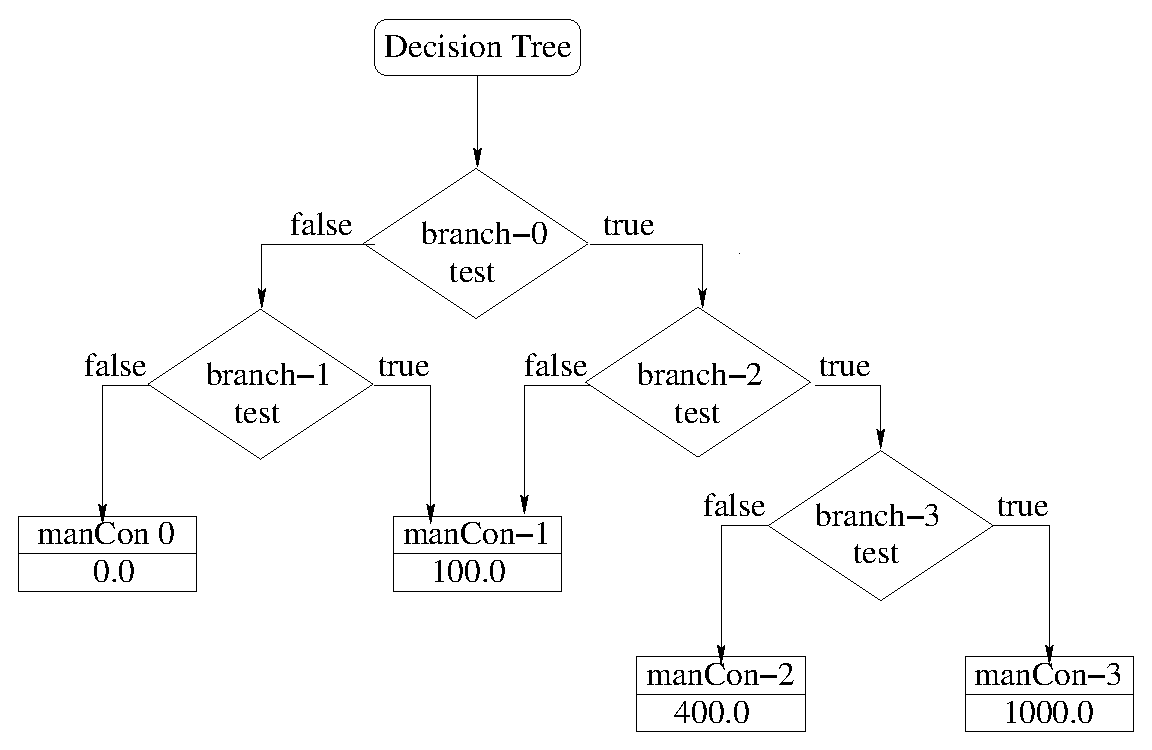
\includegraphics[scale=.45]{Graphics/flowchartDT.eps}
 \end{center}
 \caption{\label{flowchartDT} Sample Decision Tree Flowchart.}        
\end{figure}

Each branch specification contains a conditional test to
determine whether or not the hydrologic criteria has been satisfied.
If true, the {\tt true} attribute provides traversal instructions to
the decision tree manager on where to go next.  Likewise, traversal
instructions are provided by the {\tt false} attribute if the
conditional test is false.  

The RSM decision tree mechanism provides a variety of conditional tests
that can be used to test hydrologic criteria and return a Boolean
result:

\begin{enumerate}

 \item TBTest \-- the monitored value is tested against a management
 zone defined by a top and bottom rule curves.  If monitored value is
 between top and bottom, return true, otherwise return false.

 \item ABInequalityTest \-- a specified inequality (e.g., GT, GE, LT,
 LE) is used to compare a monitored value (A) with a rule curve value
 (B).  The result of the inequality test is returned.

 \item InequalityTest \-- a specified inequality (e.g., GT, GE, LT,
 LE) is used to compare a monitored value with a specified constant.
 The result of the inequality test is returned.

\end{enumerate}

The true and false traversal instructions in a branch have two parts.
The first part is either ``branch'', which indicates the next stop is
a branch, or ``manCon'', which indicates the next (and last) stop is a
management constraint.  The second part of the traversal instructions
is an integer that identifies the branch or manCon that will be processed
next. This integer must match the identification number of one of the
nested elements in decisionTree.

A management constraint is imposed on structure flow by different
processes, depending on the management method used in the RSM
implementation.

\begin{itemize}
 \item Assessor Coordinator. Every structure managed by the Assessor
   Coordinator is referenced through an MSE Node. Each MSE node
   includes management constraint variables whose values are updated
   through the deployment of MSE decision trees. The flood control and
   water supply assessors (``WCU assessors'') impose these management
   constraint variables through the course of their assessment. Since
   the WCU assessors distinquish between different purposes in their
   operational decision making, the management constraints variables
   are likewise dedicated for different purposes (e.g., flood control,
   water supply or environmental).

 \item Hydrologic Process Module. The base class for the hydrologic
   process model (HPModule) includes variables for management
   constraints whose values are updated through the deployment of HPM
   decision trees. Although these management constraint values are
   available to types of HPMs, the constraints are not applied
   generically across the HPModule classes. Currently, only the
   ModifiedSCS HPM has the capability to impose HPM decision tree
   constraints. The ModifiedSCS HPM supports the imposition of
   management constraints for flood control structure, pump and
   boundary conditions flows.

 \item Generic assessor. The MSE and HSE decision trees impose
   management constraints on flows managed within the context of
   assessor coordinators and ModifiedSCS HPMs, respectively. Other
   management methods, such as special assessors, user controllers and
   stage based operations have their own specialized ways of managing
   flows that rely on monitors to specify constraint values. Stat
   Assessor decision trees work the same as the MSE and HSE decision
   trees except they ``hold'' the management constraint variable and
   make available to other management processes through an assessor
   monitor.
\end{itemize}

The flow value used to set the management constraint can be defined by
a variety of ways.  The value or the method used to compute the value
is generally specified by the regulation schedule, policy, or
management plan simulated by regional manager.  Frequently, the
management constraint is a constant value. If the management
constraint varies by calendar date, a rule curve can be specified with
a rule curve monitor.  Other management constraints are computed,
based on the state of the system coupled with management parameters
specified by the user to simulate operational controls.  Special
purpose assessors are available to compute management constraint
values based on the current state of the system using computational
methods specified by the regulation schedule, policy or management
plan simulated by the regional manager.  These values are computed
before the regional managers are processed and access to their
computed values is provided through an assessor monitor.  Chapter
\ref{Chapter:specialPurposeAssessor} provides a description of the
special purpose assessors that can be used in conjunction with
regional managers.


